\documentclass{standalone}
\usepackage{amsmath}
\usepackage{tikz}
\usepackage{enumitem}
\usepackage[colorlinks=true]{hyperref}
\usetikzlibrary{
  arrows,
  calc,
  decorations.pathmorphing,
  decorations.pathreplacing,
  decorations.markings,
  positioning,
  shapes,
  arrows.meta
}

\ifpdf
% Ensure reproducible output
\pdfinfoomitdate=1
\pdfsuppressptexinfo=-1
\pdftrailerid{}
\hypersetup{
  pdfcreator={},
  pdfproducer={}
}
\fi

\setitemize[0]{leftmargin=15pt,itemindent=0pt,rightmargin=0pt}

\begin{document}

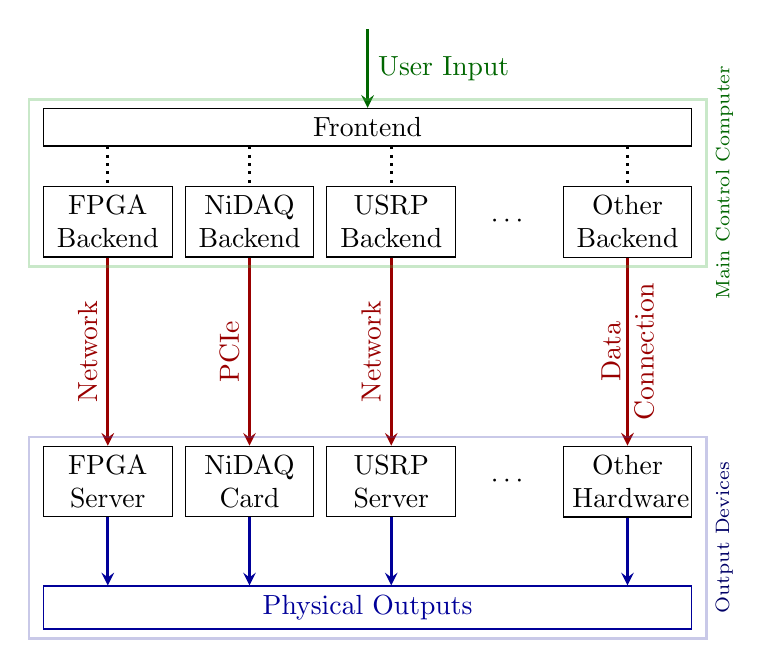
\begin{tikzpicture}
  \node[draw,text width=8cm,align=center] at (0, 0) (Frontend) {Frontend};
  \draw[->,>=stealth,line width=1,green!40!black]
  ($(Frontend.north) + (0, 1)$) -- node[right] {User Input} (Frontend.north);
  \node[draw,text width=1.4cm,align=center] at (-3.3, -1.2) (FPGA Backend) {FPGA\\Backend};
  \node[draw,text width=1.4cm,align=center] at (-1.5, -1.2) (NIDAQ Backend) {NiDAQ\\Backend};
  \node[draw,text width=1.4cm,align=center] at (0.3, -1.2) (USRP Backend) {USRP\\Backend};
  \node at (1.8, -1.2) {$\cdots$};
  \node[draw,text width=1.4cm,align=center] at (3.3, -1.2) (X Backend) {Other\\Backend};

  \draw[dotted,line width=1]
  let \p1 = (Frontend.south), \p2 = (FPGA Backend.north) in (\x2, \y1) -- (\x2, \y2);
  \draw[dotted,line width=1]
  let \p1 = (Frontend.south), \p2 = (NIDAQ Backend.north) in (\x2, \y1) -- (\x2, \y2);
  \draw[dotted,line width=1]
  let \p1 = (Frontend.south), \p2 = (USRP Backend.north) in (\x2, \y1) -- (\x2, \y2);
  \draw[dotted,line width=1]
  let \p1 = (Frontend.south), \p2 = (X Backend.north) in (\x2, \y1) -- (\x2, \y2);

  \node[draw,text width=1.4cm,align=center] at (-3.3, -4.5) (FPGA Device) {FPGA\\Server};
  \node[draw,text width=1.4cm,align=center] at (-1.5, -4.5) (NIDAQ Device) {NiDAQ\\Card};
  \node[draw,text width=1.4cm,align=center] at (0.3, -4.5) (USRP Device) {USRP\\Server};
  \node at (1.8, -4.5) {$\cdots$};
  \node[draw,text width=1.4cm,align=center] at (3.3, -4.5) (X Device) {Other\\Hardware};

  \draw[->,>=stealth,line width=1,red!60!black]
  (FPGA Backend.south) -- node[above,rotate=90] {Network} (FPGA Device.north);
  \draw[->,>=stealth,line width=1,red!60!black]
  (NIDAQ Backend.south) -- node[above,rotate=90] {PCIe} (NIDAQ Device.north);
  \draw[->,>=stealth,line width=1,red!60!black]
  (USRP Backend.south) -- node[above,rotate=90] {Network} (USRP Device.north);
  \draw[->,>=stealth,line width=1,red!60!black]
  (X Backend.south) -- node[rotate=90,align=center] {Data\\Connection} (X Device.north);

  \node[draw,text width=8cm,align=center,blue!60!black]
  at (0, -6.1) (Output) {Physical Outputs};

  \draw[->,>=stealth,line width=1,blue!60!black]
  let \p1 = (Output.north), \p2 = (FPGA Device.south) in (\x2, \y2) -- (\x2, \y1);
  \draw[->,>=stealth,line width=1,blue!60!black]
  let \p1 = (Output.north), \p2 = (NIDAQ Device.south) in (\x2, \y2) -- (\x2, \y1);
  \draw[->,>=stealth,line width=1,blue!60!black]
  let \p1 = (Output.north), \p2 = (USRP Device.south) in (\x2, \y2) -- (\x2, \y1);
  \draw[->,>=stealth,line width=1,blue!60!black]
  let \p1 = (Output.north), \p2 = (X Device.south) in (\x2, \y2) -- (\x2, \y1);

  \draw[line width=1,green!40!gray,opacity=0.3]
  let \p1 = (Frontend.north), \p2 = (FPGA Backend.south) in
  (-4.3, \y1 + 0.11cm) rectangle (4.3, \y2 - 0.11cm);
  \path let \p1 = (Frontend.north), \p2 = (FPGA Backend.south) in
  node[rotate=90,below,green!40!black] at (4.3, {(\y1 + \y2) / 2})
  {\scriptsize Main Control Computer};

  \draw[line width=1,blue!40!gray,opacity=0.3]
  let \p1 = (FPGA Device.north), \p2 = (Output.south) in
  (-4.3, \y1 + 0.11cm) rectangle (4.3, \y2 - 0.11cm);

  \path let \p1 = (FPGA Device.north), \p2 = (Output.south) in
  node[rotate=90,below,blue!40!black,align=center] at (4.3, {(\y1 + \y2) / 2})
  {\scriptsize Output Devices};
\end{tikzpicture}

\end{document}
